\iffalse

Nico Casale
Cody Orazymbetov

ECE 592 Project 1

\fi

\documentclass[]{../ncmathy}

\begin{document}
	
\section{Loading an image}
	For the project we chose an image of size 512x512, pictured below. Note that we used a grayscale image for a low-complexity implementation that computes quickly. If we used a color image, the \textit{k-means} algorithm would be passed a matrix that was $3\times$ as large, causing it to converge slowly.
	\begin{figure}[H]
		\centering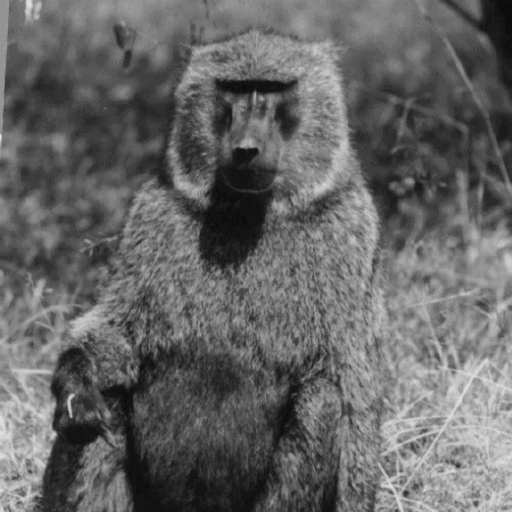
\includegraphics[width=0.5\textwidth]{image3}
		\caption{One of the images we used for the project.}
	\end{figure}
	
\section{Reconstruction of an Image with Assigned Clusters}
	\begin{figure}[H]
		\centering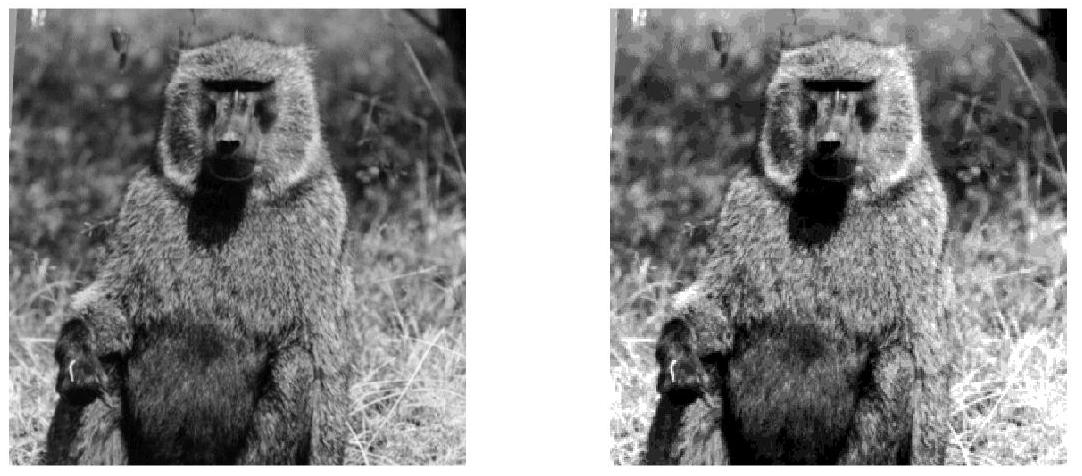
\includegraphics[width=\textwidth]{original-vs-quantized}
		\caption{The original image (left) with a quantized version (right).}
	\end{figure}
	Qualitatively, the image is recognizable and not dramatically distorted by the reconstruction. This image is the result of $P=2$ and $K=16$. 
	
\section{Rate vs. Distortion Performance}
	For this part, we chose rate R to be $[0.25, 0.5, 0.75, 1]$. To find the number of clusters given a certain rate, we used the following:
	\begin{equation}
		 C = round(2^{RP^2})
		 \label{clusters}
	\end{equation}
	Where $C$ is the number of clusters, $R$ is the coding rate, and $P$ is the patch size (in one dimension only.)  
	\\\\
	The corresponding number of clusters to the rates given is $[2, 4, 8, 16]$ for $P = 2$. The figure below illustrates the results of these variations.
	\begin{figure}[H]
		\centering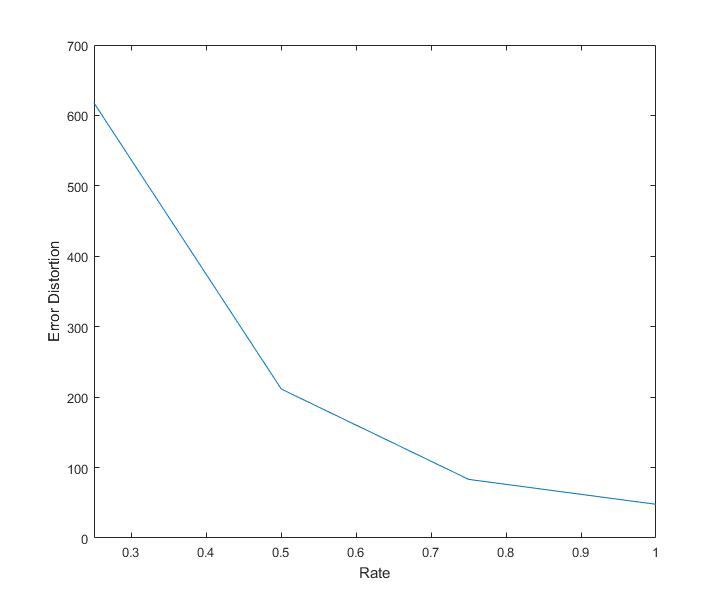
\includegraphics[width=0.6\textwidth]{RDplot}
		\caption{Rate (R) and Distortion (D) performance for patch size $P=2$}
	\end{figure} 
	The plot shows that as we increase the rate, distortion decreases. This corresponds to an increase in cluster numbers, which allows the \textit{k-means} algorithm to more accurately represent the subtleties of the image. 

\section{Varied Patch Sizes}
	As our image size is 512x512, the maximum number of clusters, which is power of 2, for the case of $P=4$ is 16384. If we used 16384 clusters, each patch of the image could be represented by its unique patch, which corresponds to the rate of 0.75. Because we cannot represent the image in more clusters than actually exist in the image, we only attempted rates from $[0.25, 0.5, 0.75]$. Below is a graph of the original RD plot with the new RD values for $P=4$.
	\begin{figure}[H]
		\centering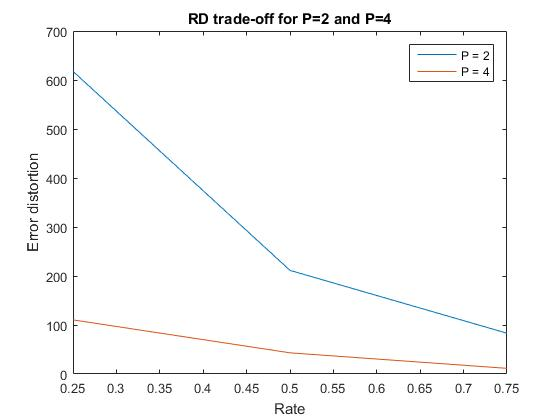
\includegraphics[width=0.6\textwidth]{rd-tradeoff-p=2,4}
		\caption{Rate (R) and Distortion (D) performance for patch size $P = 2,\ 4$}
	\end{figure}
	From the plot, we can see that even with a small rate increase we can substantially decrease the error distortion. It has a steeper drop in error when we increase the rate from 0.25 to 0.5 compared to the increase from 0.5 to 0.75. The underlying reason of getting less error with a patch size of 4 is we are having 16 components for each patch. Thus, the \textit{k-means} algorithm has more dimensions to calculate the distance to other patches. Each cluster can convey a wider range of values and capture fine-grained detail in pixel change across patch boundaries. When $P=2$ there are only 4 pixels in each patch, so the expressive capabilities of \textit{k-means} clustering is limited.
 	
\section{Better Compression with Entropy Coding}
	Being that some clusters are used more frequently to represent patches in the image, we can reduce the coding length for more likely clusters. This is similar to Morse code, where the most common letters are represented in the smallest numbers of dots and dashes. For different coding rates $R$, which correspond to the number of clusters as Eq. (\ref{clusters}),  we noticed that we could reduce the number of bits required to represent each cluster (in a normalized measure) in each case. 
	
	\begin{table}[H]
	\centering\makegapedcells
	\begin{tabular}{||c c||}
	\hline
	\thead{\makecell{R \\ (Coding Rate)}} & \thead{\makecell{Normalized Coding Length \\ (bits per pixel)}} \\
	\hline\hline
	0.25 & 0.250 \\	
	0.5 & 0.482 \\
	0.75 & 0.735 \\	
	1 & 0.962 \\ 
	\hline
	\end{tabular}
	\caption{Coding Rate vs. Normalized Coding Length with Entropy Coding.}\end{table}

	From above we can conclude the bits we use per pixel is smallest when we have a smaller cluster size ($C=2$). As we increase the cluster size, we need to use more bits to represent each cluster. Nevertheless, we can decrease the bits for 1 to 0.96 when cluster size is 16. In this configuration, we can achieve a 4\% reduction in coding rate over an implementation that does not use \textit{entropy coding}.
	
\end{document}